\section{Exercise: Estimating Time-Calibrated Phylogenies}

\subsection{Introduction}

Central among the questions explored in biology are those that seek to understand the timing and rates of evolutionary processes. Accurate estimates of species divergence times are vital to understanding historical biogeography, estimating diversification rates, and identifying the causes of variation in rates of molecular evolution. 

This tutorial will provide a general overview of divergence time estimation and fossil calibration in a Bayesian framework. The exercise will guide you through the steps necessary for estimating phylogenetic relationships and dating species divergences using the program \RevBayes. 

%\begin{figure}[h!]
%\centering
%\fbox{\includegraphics[width=3in]{figures/yule_gm.eps}}
%\caption{\small The graphical model representation of the pure-birth (Yule) process conditioned on the orgin time.}
%\label{yuleGMfig}
%\end{figure}
%

\bigskip
\subsection{Getting Started}


The various exercises in this tutorial take you through the steps required to perform phylogenetic analyses of the example datasets. 
In addition, we have provided the output files for every exercise so you can verify your results. (Note that since the MCMC runs you perform will start from different random seeds, the output files resulting from your analyses \textit{will not} be identical to the ones we provide you.)

\exs{Download data and output files from: \href{http://bit.ly/1oplDTb}{http://bit.ly/1oplDTb}
}

In this exercise, we will compare among different relaxed clock models and estimate a posterior distribution of calibrated time trees.
The dataset we will use is an alignment of 10 caniform sequences, comprising 8 bears, 1 spotted seal, and 1 gray wolf. 
Additionally, we will use occurrence times from three caniform fossils to calibrate our analysis to absolute time (Table \ref{bearFossilTable}).

\begin{table}[tbh!]
\centering
\caption{Fossil species used for calibrating divergence times in the caniform tree.}\label{bearFossilTable}
\begin{tabular}{@{\extracolsep{\fill}}l  c c c r}
\hline
\multicolumn{1}{@{}l}{\textbf{Fossil species}}  & &\multicolumn{1}{c}{\textbf{Age range (My)}}  & &\multicolumn{1}{c}{\textbf{Citation}} \\ 
\hline
\textit{Hesperocyon gregarius} & \hspace{2mm} & 37.2--40 & \hspace{2mm} & \cite{wang1994,wang1999}\\
\textit{Parictis montanus} & & 33.9--37.2 &  & \cite{clark1972,krause2008}\\
\textit{Kretzoiarctos beatrix} & & 11.2--11.8 &  & \cite{abella2011,abella12}\\
\hline
\end{tabular}
\end{table}


The alignment in file \cl{data/bears\_irbp.nex} contains interphotoreceptor retinoid-binding protein (irbp) sequences for each species.



\bigskip
\subsection{Creating Rev Files}

This tutorial sets up three different relaxed clock models and a calibrated birth-death model. 
Because of the complexity of the various models, this exercise is best performed by specifying the models and samplers in different \Rev~files.
At the beginning of each section, you will be given a suggested name for each component file; these names correspond to the provided \Rev~scripts that reproduce these commands.
 


\bigskip
\subsection{Calibrating the Birth-Death Model}\label{brMods} 

Fortunately, the fossil record for caniforms (and other carnivores) is quite good. 
We must formulate a birth-death model that accounts for the fossil occurrence times in Table \ref{bearFossilTable}. 
This part of the exercise will involve specifying a birth-death model with clamped stochastic nodes representing the observation times of two fossils descended from internal nodes in our tree: (1) \textit{Parictis montanus}, the oldest fossil in the family Ursidae, a stem fossil bear, and (2) \textit{Kretzoiarctos beatrix}, the fossil Ailuropodinae, a crown fossil bear.
Additionally, we will use the canid fossil, \textit{Hesperocyon gregarius}, to offset the age of the root of the tree. 

In \RevBayes, calibrated internal nodes are treated differently than in many other programs for estimating species divergence times (e.g., BEAST).
This is because the graphical model structure used in \RevBayes~does not allow a stochastic node to be assigned more than one prior distribution. 
By contrast, the common approach to applying calibration densities as used in other dating softwares leads to incoherence in the calibration prior \citep{warnock12,heled12,heath2013fossilized}. 
More explicitly, common calibration approaches assume that the age of a calibrated node is modeled by the tree-wide diversification process (e.g., birth-death model) \textit{and} a parametric density parameterized by the occurrence time of a fossil (or other external prior information).
This can induce a calibration prior density that is not consistent with the birth-death process or the parametric prior distribution. 
Thus, approaches that condition the birth-death process on the calibrated nodes are more statistically coherent \citep{yang06}.

In \RevBayes, calibration densities are applied in a different way, treating fossil observation times like data. 
The graphical model in Figure \ref{m_BDCal:fig} illustrates how calibrated nodes are specified in the directed acyclic graph (DAG).
Here, the age of the calibration node (i.e., the internal node specified as the MRCA of the fossil and a set of living species) is a deterministic node---e.g., denoted $o_1$ for fossil $\mathcal{F}_1$---and acts as an offset on the stochastic node representing the age of the fossil specimen.
The fossil age, $\mathcal{F}_i$, is specified as a stochastic node and clamped to its \textit{observed} age in the fossil record. 
The node $\mathcal{F}_i$ is modeled using a distribution that describes the waiting time from the speciation event to the appearance of the observed fossil. 
Thus, if the MCMC samples any state of $\Psi$ for which the age of $\mathcal{F}_i$ has a probability of 0, then that state will always be rejected, effectively calibrating the birth-death process without applying multiple prior densities to any calibrated node (Fig.~\ref{m_BDCal:fig}).

The root age is treated differently, however. 
Here, we condition the birth-death process on the speciation time of the root, thus this variable is not part of the time-tree parameter. 
The root age can thus be given any parametric distribution over positive real numbers (Fig.~\ref{m_BDCal:fig}).

\begin{figure}[h!]
\centering
\fbox{\includegraphics[width=6in]{figures/calib_BDR_gm.eps}}
\caption{\small The graphical model representation of the node-calibrated birth-death process in \RevBayes.}
\label{m_BDCal:fig}
\end{figure}

\textbf{\textit{Create the Rev File}}

{\begin{framed}
Open your text editor and create the birth-death model file called {\textcolor{red}{\cl{m\_BDP\_Tree\_bears.Rev}}} in the \cl{RevBayes\_scripts} directory.

Enter the \Rev~code provided in this section in the new model file.
\end{framed}}


\textbf{\textit{Read in the Starting Tree}}

When calibrating nodes in the birth-death process, it is very helpful to have a starting tree that is consistent with the topology constraints and calibration priors, otherwise, the probability of the model would be 0 and the MCMC cannot run.
For a starting tree we will use the tree estimated by \citet{dosReis2012}. 
{\tt \begin{snugshade*}
\begin{lstlisting}
T <- readTrees("data/bears_dosReis.tre")[1]
\end{lstlisting}
\end{snugshade*}}

From the tree we can initialize some useful variables.
{\tt \begin{snugshade*}
\begin{lstlisting}
n_taxa <- T.ntips()
names <- T.names()
\end{lstlisting}
\end{snugshade*}}

%And our move-index iterator.
%{\tt \begin{snugshade*}
%\begin{lstlisting}
%mi <- 0
%\end{lstlisting}
%\end{snugshade*}}

\subsubsection{Birth-Death Parameters}

We will begin by setting up the model parameters and proposal mechanisms of the birth-death model. 
Note that we have not initialized the workspace iterator \cl{mi} yet. 
Because of this, if you typed these lines in \RevBayes, you would get an error. 
Since this code is intended to be in a sourced \Rev~file, we are assuming that you would initialize \cl{mi} before calling \cl{source("RevBayes\_scripts/m\_BDP\_Tree\_bears.Rev")}.

\textbf{\textit{Diversification}}
{\tt \begin{snugshade*}
\begin{lstlisting}
diversification ~ dnExponential(10.0) 
moves[mi++] <- mvScale(diversification,lambda=1.0,tune=true,weight=3.0)
\end{lstlisting}
\end{snugshade*}}

\textbf{\textit{Turnover}}
{\tt \begin{snugshade*}
\begin{lstlisting}
turnover ~ dnBeta(2.0, 2.0) 
moves[mi++] <- mvSlide(turnover,delta=1.0,tune=true,weight=3.0)
\end{lstlisting}
\end{snugshade*}}

\textbf{\textit{Deterministic Nodes for Birth and Death Rates}}

The birth rate and death rate are deterministic functions of the diversification and turnover.
First, create a deterministic node for $1 - r$, which is the denominator for each formula.

{\tt \begin{snugshade*}
\begin{lstlisting}
denom := abs(1.0 - turnover) 
\end{lstlisting}
\end{snugshade*}}

Now, the rates will both be positive real numbers that are variable transformations of the stochastic variables.
{\tt \begin{snugshade*}
\begin{lstlisting}
birth_rate := diversification / (denom)
death_rate := (turnover * diversification) / (denom)
\end{lstlisting}
\end{snugshade*}}

\textbf{\textit{Sampling Probability}}

Fix the probability of sampling to a known value. Since there are approximately 147 described caniform species, we will create a constant node for this parameter.
{\tt \begin{snugshade*}
\begin{lstlisting}
rho <- 0.068
\end{lstlisting}
\end{snugshade*}}

\subsubsection{Prior on the Root Node}

The fossil \textit{Hesperocyon gregarius} is a fossil descendant of the most-recent common ancestor of all caniformes and has an occurrence time of $\sim$38 Mya.
Thus, we can assume that the probability of the root age being younger than 38 Mya is equal to 0, using this value to offset a prior distribution on the root-age.

First specify the occurrence-time of the fossil.
{\tt \begin{snugshade*}
\begin{lstlisting}
tHesperocyon <- 38.0
\end{lstlisting}
\end{snugshade*}}

We will assume a lognormal prior on the root age that is offset by the observed age of \textit{Hesperocyon gregarius}. 
We can use the previous analysis by \citet{dosReis2012} to parameterize the lognormal prior on the root time. 
The age for the MRCA of the caniformes reported in their study was $\sim$49 Mya. 
Therefore, we can specify the mean of our lognormal distribution to equal $49 - 38 = 11$ Mya.
Given the expected value of the lognormal (\cl{mean\_ra}) and a standard deviation (\cl{stdv\_ra}), we can also compute the location parameter of the lognormal (\cl{mu\_ra}).
{\tt \begin{snugshade*}
\begin{lstlisting}
mean_ra <- 11.0
stdv_ra <- 0.25
mu_ra <- ln(mean_ra) - ((stdv_ra*stdv_ra) * 0.5)
\end{lstlisting}
\end{snugshade*}}

With these parameters we can instantiate the root age stochastic node with the offset value.
{\tt \begin{snugshade*}
\begin{lstlisting}
root_time ~ dnLnorm(mu_ra, stdv_ra, offset=tHesperocyon)
\end{lstlisting}
\end{snugshade*}}


\subsubsection{Topology Constraints \& Time Tree}

To create the tree with calibrated nodes, we must constrain the topology such that the calibrated nodes always have the same descendants.

The two non-root nodes we are calibrating in this tree is the MRCA of all living bears:
{\tt \begin{snugshade*}
\begin{lstlisting}
clade_Ursidae <- clade("Ailuropoda_melanoleuca","Tremarctos_ornatus","Helarctos_malayanus", "Ursus_americanus","Ursus_thibetanus","Ursus_arctos","Ursus_maritimus","Melursus_ursinus")
\end{lstlisting}
\end{snugshade*}}

And the MRCA of all bears and pinnipeds. 
{\tt \begin{snugshade*}
\begin{lstlisting}
clade_UrsPinn <- clade("Ailuropoda_melanoleuca","Tremarctos_ornatus","Helarctos_malayanus", "Ursus_americanus","Ursus_thibetanus","Ursus_arctos","Ursus_maritimus","Melursus_ursinus", "Phoca_largha")
\end{lstlisting}
\end{snugshade*}}

Once we have a set of constraints, we can use the vector function \cl{v()} to bind them in a constant vector.
{\tt \begin{snugshade*}
\begin{lstlisting}
constraints <- v(clade_Ursidae, clade_UrsPinn)
\end{lstlisting}
\end{snugshade*}}

Now we have all of the elements needed to specify the time-tree parameter.
{\tt \begin{snugshade*}
\begin{lstlisting}
timetree ~ dnBDP(lambda=birth_rate, mu=death_rate, rho=rho, rootAge=root_time, samplingStrategy="uniform", condition="nTaxa", nTaxa=n_taxa, names=names,constraints=constraints)
\end{lstlisting}
\end{snugshade*}}


\subsubsection{Calibrating Constrained Nodes}

In order that our tree is consistent with the calibration ages, we must first set the value of the time-tree node to our starting tree.
{\tt \begin{snugshade*}
\begin{lstlisting}
timetree.setValue(T)
\end{lstlisting}
\end{snugshade*}}

To begin specifying the calibration density on the MRCA of all ursids, we must first create the deterministic node representing the age of the MRCA.
The way in which these densities work requires the offset to be negative. 
Therefore we are creating two deterministic variables, one positive for monitoring, and one negative for the off-set.
We use the \cl{tmrca()} function to create these nodes which require that you provide a clade constraint.
{\tt \begin{snugshade*}
\begin{lstlisting}
tmrca_Ursidae := tmrca(timetree,clade_Ursidae)
n_TMRCA_Ursidae := -(tmrca_Ursidae)
\end{lstlisting}
\end{snugshade*}}

Now, we must specify our fossil occurrence time.
This is the age for the fossil panda, \textit{Kretzoiarctos beatrix}.
Note that we also make this value negative.
{\tt \begin{snugshade*}
\begin{lstlisting}
tKretzoiarctos <- -11.2
\end{lstlisting}
\end{snugshade*}}

Create the stochastic node for the age of the crown ursid fossil, using a lognormal distribution.
{\tt \begin{snugshade*}
\begin{lstlisting}
M <- 10
sdv <- 0.25
mu <- ln(M) - ((sdv * sdv) * 0.5)
crown_Ursid_fossil ~ dnLnorm(mu, sdv, offset=n_TMRCA_Ursidae)
\end{lstlisting}
\end{snugshade*}}

Now clamp the fossil age stochastic node with the observation time of \textit{Kretzoiarctos beatrix}
{\tt \begin{snugshade*}
\begin{lstlisting}
crown_Ursid_fossil.clamp(tKretzoiarctos)
\end{lstlisting}
\end{snugshade*}}

Next we will create the variable for the age of the MRCA of all bears and pinnipeds.
{\tt \begin{snugshade*}
\begin{lstlisting}
tmrca_UrsidaePinn := tmrca(timetree,clade_UrsPinn)
n_TMRCA_UrsidaePinn := -(tmrca_UrsidaePinn)
\end{lstlisting}
\end{snugshade*}}

Set the observed time for the stem fossil bear.
{\tt \begin{snugshade*}
\begin{lstlisting}
tParictis <- -33.9
\end{lstlisting}
\end{snugshade*}}

Create the stochastic node using the exponential prior and clamp it with the observation time of the fossil.
{\tt \begin{snugshade*}
\begin{lstlisting}
stem_Ursid_fossil ~ dnExponential(lambda=0.0333, offset=n_TMRCA_UrsidaePinn)
stem_Ursid_fossil.clamp(tParictis)
\end{lstlisting}
\end{snugshade*}}

\subsubsection{Proposals on the Time Tree}

Next, create the vector of moves. These tree moves act on node ages:
{\tt \begin{snugshade*}
\begin{lstlisting}
moves[mi++] <- mvNodeTimeSlideUniform(timetree, weight=30.0)
moves[mi++] <- mvSlide(root_time, delta=2.0, tune=true, weight=10.0)
moves[mi++] <- mvScale(root_time, lambda=2.0, tune=true, weight=10.0)
moves[mi++] <- mvTreeScale(tree=timetree, rootAge=root_time, delta=1.0, tune=true, weight=3.0)
\end{lstlisting}
\end{snugshade*}}

And these change the tree topology. If we wish to keep the topology constant, then we can leave these moves out. Note that for some relaxed clock models (autocorrelated rates, DPP, random-local clock) tree topology moves often induce very long mixing times.
{\tt \begin{snugshade*}
\begin{lstlisting}
moves[mi++] <- mvNNI(timetree, weight=8.0)
moves[mi++] <- mvNarrow(timetree, weight=8.0)
moves[mi++] <- mvFNPR(timetree, weight=8.0)
\end{lstlisting}
\end{snugshade*}}



\bigskip
\subsection{Specifying Branch-Rate Models}\label{brMods} 

The next sections will walk you through setting up the files specifying different relaxed clock models. 
You may type this syntax directly into the \RevBayes~console or write them in a text file.

\bigskip
\subsubsection{The Global Molecular Clock Model}

The global molecular clock assumes that the rate of substitution is constant over the tree and over time.
When estimating trees on an absolute time-scale, it is often necessary to parameterize relaxed clock models with two rates, a base rate which effectively scales the tree and a clock rate. 
Then, the absolute rate applied to the tree is a deterministic node (Fig.~\ref{m_GMC:fig}).

\begin{figure}[h!]
\centering
\fbox{\includegraphics[width=3in]{figures/gmc_gm.eps}}
\caption{\small The graphical model representation of the global molecular clock model used in this exercise.}
\label{m_GMC:fig}
\end{figure}


\textbf{\textit{Load Sequence Alignment}}

Read in the sequences and initialize important variables.
{\tt \begin{snugshade*}
\begin{lstlisting}
D <- readCharacterData(file="data/bears_irbp.nex")
n_sites <- D.nchar(1)
mi <- 0
\end{lstlisting}
\end{snugshade*}}

\textbf{\textit{The Calibrated Time-Tree Model}}

Load the calibrated tree model from file. Note that this file does not have moves that operate on the tree topology, which is helpful when you plan to estimate the marginal likelihoods and compare different relaxed clock models.
{\tt \begin{snugshade*}
\begin{lstlisting}
source("RevBayes_scripts/m_BDP_bears.Rev")
\end{lstlisting}
\end{snugshade*}}

\textbf{\textit{The Clock-Rate}}

We specify the absolute clock rate by first creating a node for the base rate.
This value is set to be drawn from a lognormal prior.
{\tt \begin{snugshade*}
\begin{lstlisting}
br_M <- 5.4E-3
br_s <- 0.05
br_mu <- ln(br_M) - ((br_s * br_s) * 0.5)
base_rate ~ dnLnorm(br_mu, br_s)
moves[mi++] <- mvScale(base_rate,lambda=0.25,tune=true,weight=5.0)
\end{lstlisting}
\end{snugshade*}}

The clock-rate parameter is a stochastic node from a gamma distribution.
{\tt \begin{snugshade*}
\begin{lstlisting}
clock_rate ~ dnGamma(2.0,4.0)
moves[mi++] <- mvScale(clock_rate,lambda=0.5,tune=true,weight=5.0)
\end{lstlisting}
\end{snugshade*}}

The absolute clock rate is the value on which the phylogenetic CTMC model depends. This is a deterministic node and equal to the product of the base rate and clock rate.
{\tt \begin{snugshade*}
\begin{lstlisting}
abs_clock_rt := clock_rate * base_rate
\end{lstlisting}
\end{snugshade*}}

\textbf{\textit{The Sequence Model and Tree Plate}}

Specify the parameters of the GTR model and the moves to operate on them.
{\tt \begin{snugshade*}
\begin{lstlisting}
sf ~ dnDirichlet(v(1,1,1,1))
er ~ dnDirichlet(v(1,1,1,1,1,1))
Q := gtr(er,sf)
moves[mi++] <- mvSimplexElementScale(er, alpha=10.0, tune=true, weight=3.0)
moves[mi++] <- mvSimplexElementScale(sf, alpha=10.0, tune=true, weight=3.0)
\end{lstlisting}
\end{snugshade*}}

And instantiate the phyoCTMC.
{\tt \begin{snugshade*}
\begin{lstlisting}
phySeq ~ dnPhyloCTMC(tree=timetree, Q=Q, branchRates=abs_clock_rt, nSites=n_sites, type="DNA")
phySeq.clamp(D)
\end{lstlisting}
\end{snugshade*}}

Specify the work-space model object.
{\tt \begin{snugshade*}
\begin{lstlisting}
mymodel <- model(er)
\end{lstlisting}
\end{snugshade*}}

\exs{The global-molecular clock model is specified in the file called \href{https://github.com/revbayes/revbayes/raw/development/tutorials/RB_TimeTree_Tutorials/RB_TimeTree_Exercise/RB_timetree_files/RevBayes_scripts/m_GMC_bears.Rev}{\cl{m\_GMC\_bears.Rev }}.}

\textbf{\textit{Estimate the Marginal Likelihood}}

Below is the code to estimate the marginal likelihood. 
Enter the value for this model in Table \ref{ssTable}.

\exs{The strict clock marginal likelihood analysis is specified in the file called \href{https://github.com/revbayes/revbayes/raw/development/tutorials/RB_TimeTree_Tutorials/RB_TimeTree_Exercise/RB_timetree_files/RevBayes_scripts/mlnl_GMC_bears.Rev}{\cl{mlnl\_GMC\_bears.Rev }}.}

{\tt \begin{snugshade*}
\begin{lstlisting}
source("RevBayes_scripts/m_GMC_bears.Rev")

pow_p <- powerPosterior(mymodel, moves, "output/GMC_bears_powp.out", cats=50) 
pow_p.burnin(generations=5000,tuningInterval=200)
pow_p.run(generations=1000)  

ss <- steppingStoneSampler(file="output/GMC_bears_powp.out", powerColumnName="power", likelihoodColumnName="likelihood")
ss.marginal() 

### use path sampling to calculate marginal likelihoods
ps <- pathSampler(file="output/GMC_bears_powp.out", powerColumnName="power", likelihoodColumnName="likelihood")
ps.marginal() 
\end{lstlisting}
\end{snugshade*}}


\bigskip
\subsubsection{The Uncorrelated Lognormal Rates Model}

The uncorrelated lognormal model relaxes the assumption of a single-rate molecular clock. 
Under this model, the rate associated with each branch in the tree is a stochastic node.
Each branch-rate variable is drawn from the same lognormal distribution (Fig.~\ref{m_UCLN:fig}).

Given that we might not have prior information on the parameters of the lognormal distribution, we can assign hyper priors to these variables. 
Generally, it is more straightforward to construct a hyperprior on the expectation (i.e., the mean) of a lognormal density rather than the location parameter $\mu$. 
Here, we will assume that the mean branch rate is exponentially distributed and as is the stochastic node representing the standard deviation.
With these two parameters, we can get the location parameter of the lognormal by:
$$\mu = \log(M) - \frac{\sigma^2}{2}.$$
Thus, $\mu$ is a deterministic node, which is a function of $M$ and $\sigma$.

In Figure \ref{m_UCLN:fig}, we can represent the vector of $N$ branch rates using the plate notation. Additionally, each branch rate is rescaled by the base rate. 
\begin{figure}[h!]
\centering
\fbox{\includegraphics[width=3in]{figures/ucln_gm.eps}}
\caption{\small The graphical model representation of the UCLN model used in this exercise.}
\label{m_UCLN:fig}
\end{figure}

First, clear the workspace.
{\tt \begin{snugshade*}
\begin{lstlisting}
clear()
\end{lstlisting}
\end{snugshade*}}


\textbf{\textit{Load the Sequence Data and Birth-Death Model}}

{\tt \begin{snugshade*}
\begin{lstlisting}
D <- readCharacterData(file="data/bears_irbp.nex")
n_sites <- D.nchar(1)
mi <- 0
\end{lstlisting}
\end{snugshade*}}

{\tt \begin{snugshade*}
\begin{lstlisting}
source("RevBayes_scripts/m_BDP_bears.Rev")
\end{lstlisting}
\end{snugshade*}}

\textbf{\textit{The Base Clock Rate}}

As in the clock model above, we create a lognormally distributed stochastic node, representing the base rate.
{\tt \begin{snugshade*}
\begin{lstlisting}
br_M <- 5.4E-3
br_s <- 0.05
br_mu <- ln(br_M) - ((br_s * br_s) * 0.5)
base_rate ~ dnLnorm(br_mu, br_s)
moves[mi++] <- mvScale(base_rate,lambda=0.25,tune=true,weight=5.0)
\end{lstlisting}
\end{snugshade*}}

\textbf{\textit{Independent Branch Rates}}

Before we can set up the variable of the branch-rate model, we must know how many branches exist in the tree.
{\tt \begin{snugshade*}
\begin{lstlisting}
n_branches <- 2 * n_taxa - 2
\end{lstlisting}
\end{snugshade*}}

We will start with the mean of the lognormal distribution, $M$ in Figure \ref{m_UCLN:fig}.
{\tt \begin{snugshade*}
\begin{lstlisting}
ucln_mean ~ dnExponential(2.0)
\end{lstlisting}
\end{snugshade*}}

And the exponentially distributed node representing the standard deviation.
We will also create a deterministic node, which is the variance, $\sigma^2$.
{\tt \begin{snugshade*}
\begin{lstlisting}
ucln_sigma ~ dnExponential(3.0)
ucln_var := ucln_sigma * ucln_sigma
\end{lstlisting}
\end{snugshade*}}

Now we can declare the function that gives us the $\mu$ parameter of the lognormal distribution on branch rates.
{\tt \begin{snugshade*}
\begin{lstlisting}
ucln_mu := ln(ucln_mean) - (ucln_var * 0.5)
\end{lstlisting}
\end{snugshade*}}

The only stochastic nodes we need to operate on for this part of the model are the lognormal mean ($M$ or \cl{ucln\_mean}) and the standard deviation ($\sigma$ or \cl{ucln\_sigma}).
{\tt \begin{snugshade*}
\begin{lstlisting}
moves[mi++] <- mvScale(ucln_mean, lambda=1.0, tune=true, weight=4.0)
moves[mi++] <- mvScale(ucln_sigma, lambda=0.5, tune=true, weight=4.0)
\end{lstlisting}
\end{snugshade*}}

With our nodes representing the $\mu$ and $\sigma$ of the lognormal distribution, we can create the vector of stochastic nodes for each of the branch rates using a \cl{for} loop. 
Within this loop, we also add the move for each branch-rate stochastic node to our moves vector.
{\tt \begin{snugshade*}
\begin{lstlisting}
for(i in 1:n_branches){
   branch_rates[i] ~ dnLnorm(ucln_mu, ucln_sigma)
   moves[mi++] <- mvScale(branch_rates[i], lambda=1, tune=true, weight=2.)
}
\end{lstlisting}
\end{snugshade*}}

Because we are dealing with semi-identifiable parameters, it often helps to apply a range of moves to the variables representing the branch rates and branch times. This will help to improve the mixing of our MCMC.
Here we will add 2 additional types of moves that act on vectors.
{\tt \begin{snugshade*}
\begin{lstlisting}
moves[mi++] <- mvVectorScale(branch_rates,lambda=1.0,tune=true,weight=2.0) 
moves[mi++] <- mvVectorSingleElementScale(branch_rates,lambda=30.0,tune=true,weight=1.0) 
\end{lstlisting}
\end{snugshade*}}

We can combine the base rate and branch rates in a vector of deterministic nodes.
{\tt \begin{snugshade*}
\begin{lstlisting}
branch_subrates := branch_rates * base_rate
\end{lstlisting}
\end{snugshade*}}

The mean of the branch rates is a convenient deterministic node to monitor, particularly in the screen output when conducting MCMC.
{\tt \begin{snugshade*}
\begin{lstlisting}
mean_rt := mean(branch_rates) 
\end{lstlisting}
\end{snugshade*}}

\textbf{\textit{The Sequence Model and Tree Plate}}

Now, specify the stationary frequencies and exchangeability rates of the GTR matrix.
{\tt \begin{snugshade*}
\begin{lstlisting}
sf ~ dnDirichlet(v(1,1,1,1))
er ~ dnDirichlet(v(1,1,1,1,1,1))
Q := gtr(er,sf)
moves[mi++] <- mvSimplexElementScale(er, alpha=10.0, tune=true, weight=3.0)
moves[mi++] <- mvSimplexElementScale(sf, alpha=10.0, tune=true, weight=3.0)
\end{lstlisting}
\end{snugshade*}}

Now, we can put the whole model together in the phylogenetic CTMC and clamp that node with our sequence data.
{\tt \begin{snugshade*}
\begin{lstlisting}
phySeq ~ dnPhyloCTMC(tree=timetree, Q=Q, branchRates=branch_subrates, nSites=n_sites, type="DNA")
attach the observed sequence data
phySeq.clamp(D)
\end{lstlisting}
\end{snugshade*}}

{\tt \begin{snugshade*}
\begin{lstlisting}
mymodel <- model(er)
\end{lstlisting}
\end{snugshade*}}

\exs{The UCLN model is specified in the file called \href{https://github.com/revbayes/revbayes/raw/development/tutorials/RB_TimeTree_Tutorials/RB_TimeTree_Exercise/RB_timetree_files/RevBayes_scripts/m_UCLN_bears.Rev}{\cl{m\_UCLN\_bears.Rev }}.}

\textbf{\textit{Estimate the Marginal Likelihood}}

Below is the code to estimate the marginal likelihood. 
Enter the value for this model in Table \ref{ssTable}.

\exs{The UCLN marginal likelihood analysis is specified in the file called \href{https://github.com/revbayes/revbayes/raw/development/tutorials/RB_TimeTree_Tutorials/RB_TimeTree_Exercise/RB_timetree_files/RevBayes_scripts/mlnl_UCLN_bears.Rev}{\cl{mlnl\_UCLN\_bears.Rev }}.}

{\tt \begin{snugshade*}
\begin{lstlisting}
source("RevBayes_scripts/m_GMC_bears.Rev")

pow_p <- powerPosterior(mymodel, moves, "output/UCLN_bears_powp.out", cats=50) 
pow_p.burnin(generations=5000,tuningInterval=200)
pow_p.run(generations=1000)  

ss <- steppingStoneSampler(file="output/UCLN_bears_powp.out", powerColumnName="power", likelihoodColumnName="likelihood")
ss.marginal() 

### use path sampling to calculate marginal likelihoods
ps <- pathSampler(file="output/GMC_bears_powp.out", powerColumnName="power", likelihoodColumnName="likelihood")
ps.marginal() 
\end{lstlisting}
\end{snugshade*}}


\FloatBarrier
\subsection{Compute Bayes Factors and Select Model}


Now that we have estimates of the marginal likelihood under each of our different models, we can evaluate their relative plausibility using Bayes factors.
Use Table \ref{ssTable} to summarize the marginal log-likelihoods estimated using the stepping-stone and path-sampling methods.
\begin{Form}
\begin{table}[h!]
\centering
\caption{\small Estimated marginal likelihoods for different partition configurations$^*$.}
\begin{tabular}{l c c c c}
\hline
\multicolumn{1}{l}{\textbf{ }} &\multicolumn{1}{r}{\textbf{ }} & \multicolumn{3}{c}{\textbf{Marginal lnL estimates}} \\ 
\cline{3-5}
\multicolumn{1}{l}{\textbf{Partition}} & \multicolumn{1}{r}{\hspace{3mm}} & \multicolumn{1}{c}{\textit{Stepping-stone}} & \multicolumn{1}{r}{\hspace{3mm}} & \multicolumn{1}{c}{\textit{Path sampling}} \\ 
\hline
Global molecular clock ($M_0$) & \hspace{15mm} & \TextField[name=m1,backgroundcolor={.85 .85 .85},color={1 0 0},height=4ex]{}  & \hspace{15mm} & \TextField[name=ml2,backgroundcolor={.85 .85 .85},color={0 0 1},height=4ex]{} \\
\hline
Uncorrelated lognormal ($M_1$) & \hspace{3mm} &\TextField[name=ml3,backgroundcolor={.85 .85 .85},color={1 0 0},height=4ex]{}   & \hspace{3mm} & \TextField[name=ml4,backgroundcolor={.85 .85 .85},color={0 0 1},height=4ex]{} \\
\hline
%\ref{mlnl_ACLN} Autocorrelated lognormal  ($M_2$) & \hspace{3mm} & \TextField[name=ml5,backgroundcolor={.85 .85 .85},color={1 0 0},height=4ex]{} & \hspace{3mm} & \TextField[name=ml6,backgroundcolor={.85 .85 .85},color={0 0 1},height=4ex]{} \\
{\footnotesize{$^*$you can edit this table}}\\
\end{tabular}
\label{ssTable}
\end{table}
\end{Form}

Phylogenetics software programs log-transform the likelihood to avoid \href{http://en.wikipedia.org/wiki/Arithmetic_underflow}{underflow}, because multiplying likelihoods results in numbers that are too small to be held in computer memory.
Thus, we must calculate the ln-Bayes factor (we will denote this value $\mathcal{K}$):
\begin{align}\label{LNbfFormula}
\mathcal{K}=\ln[BF(M_0,M_1)] = \ln[\mathbb{P}(\mathbf X \mid M_0)]-\ln[\mathbb{P}(\mathbf X \mid M_1)],
\end{align}
where $\ln[\mathbb{P}(\mathbf X \mid M_0)]$ is the \textit{marginal lnL} estimate for model $M_0$. 
The value resulting from equation \ref{LNbfFormula} can be converted to a raw Bayes factor by simply taking the exponent of $\cal{K}$
\begin{align}\label{LNbfFormula2}
BF(M_0,M_1) = e^{\cal{K}}.
\end{align}
Alternatively, you can interpret the strength of evidence in favor of $M_0$ using the $\cal{K}$ and skip equation \ref{LNbfFormula2}. 
In this case, we evaluate the $\cal{K}$ in favor of model $M_0$ against model $M_1$ so that:
\begin{center}
\begin{tabular}{l}
if $\mathcal{K} > 1$, then model $M_0$ wins\\
if $\mathcal{K} < -1$, then model $M_1$ wins.
\end{tabular}
\end{center}
Thus, values of $\mathcal{K}$ around 0 indicate ambiguous support. 


Using the values you entered in Table \ref{ssTable} and equation \ref{LNbfFormula},  calculate the ln-Bayes factors (using $\mathcal{K}$) for the different model comparisons. 
Enter your answers in Table \ref{bfTable} using the stepping-stone and the path-sampling estimates of the marginal log likelihoods. 

\begin{Form}
\begin{table}[h!]
\centering
\caption{\small Bayes factor calculation$^*$.}
\begin{tabular}{l c c c c}
\hline
\multicolumn{1}{l}{\textbf{ }} &\multicolumn{1}{r}{\textbf{ }} & \multicolumn{3}{c}{\textbf{ln-Bayes Factor} ($\mathcal{K}$)} \\ 
\cline{3-5}
\multicolumn{1}{l}{\textbf{Model comparison}} & \multicolumn{1}{r}{\hspace{3mm}} & \multicolumn{1}{c}{\textit{Stepping-stone}} & \multicolumn{1}{r}{\hspace{3mm}} & \multicolumn{1}{c}{\textit{Path sampling}} \\ 
\hline
$M_0,M_1$ & \hspace{15mm} & \TextField[name=ml7,backgroundcolor={.85 .85 .85},color={1 0 0},height=4ex]{}  & \hspace{15mm} & \TextField[name=ml8,backgroundcolor={.85 .85 .85},color={0 0 1},height=4ex]{} \\
\hline
Supported model? & \hspace{3mm} &  \TextField[name=ml13,backgroundcolor={1 .85 .85},color={1 0 0},height=4ex]{} & \hspace{3mm} & \TextField[name=ml14,backgroundcolor={.85 .85 1},color={0 0 1},height=4ex]{} \\
\hline
{\footnotesize{$^*$you can edit this table}}\\
\end{tabular}
\label{bfTable}
\end{table}
\end{Form}

\bigskip
\subsection{Estimate the Topology and Branch Times}

Below the code is provided to run the MCMC analysis under the UCLN model while estimating the topology and branching times.

{\tt \begin{snugshade*}
\begin{lstlisting}

### Load the sequence alignment
D <- readCharacterData(file="data/bears_irbp.nex")

### get helpful variables from the data
n_taxa <- D.ntaxa()
n_sites <- D.nchar(1)
names <- D.names()

### initialize an iterator for the moves vector
mi <- 0

### set up the birth-death model from file
### this file includes tree topology moves
source("RevBayes_scripts/m_BDP_Tree_bears.Rev")

####################################
############ UCLN model ###########
###################################

source("RevBayes_scripts/m_UCLN_bears.Rev")

\end{lstlisting}
\end{snugshade*}}

Set up the MCMC
{\tt \begin{snugshade*}
\begin{lstlisting}

### workspace model wrapper ###
mymodel <- model(er)

monitors[1] <- mnFile(filename="output/TimeTree_bears_mcmc.log", printgen=10,diversification, turnover, birth_rate, death_rate, root_time, tmrca_Ursidae, tmrca_UrsidaePinn,er, sf,mean_rt, ucln_mean, ucln_sigma, branch_rates, base_rate)
monitors[2] <- mnFile(filename="output/TimeTree_bears_mcmc.trees", printgen=10, timetree)
monitors[3] <- mnScreen(printgen=10, mean_rt, ucln_mean, root_time, base_rate)

### workspace mcmc ###
mymcmc <- mcmc(mymodel, monitors, moves)

### pre-burnin to tune the proposals ###
mymcmc.burnin(generations=3000,tuningInterval=100)

### run the MCMC ###
mymcmc.run(generations=50000)

### display proposal acceptance rates and tuning ###
mymcmc.operatorSummary()

\end{lstlisting}
\end{snugshade*}}

Summarize the tree
{\tt \begin{snugshade*}
\begin{lstlisting}

### summarize the trees ###
tt <- readTreeTrace("output/TimeTree_bears_mcmc.trees", "clock")
tt.summarize()

### write MAP tree to file
mapTree(tt, "output/TimeTree_bears_mcmc_MAP.tre")

## quit ##
q()
\end{lstlisting}
\end{snugshade*}}

%{\tt \begin{snugshade*}
%\begin{lstlisting}
%
%\end{lstlisting}
%\end{snugshade*}}
%
%{\tt \begin{snugshade*}
%\begin{lstlisting}
%
%\end{lstlisting}
%\end{snugshade*}}
%
%{\tt \begin{snugshade*}
%\begin{lstlisting}
%
%\end{lstlisting}
%\end{snugshade*}}
%
%{\tt \begin{snugshade*}
%\begin{lstlisting}
%
%\end{lstlisting}
%\end{snugshade*}}
%
%{\tt \begin{snugshade*}
%\begin{lstlisting}
%
%\end{lstlisting}
%\end{snugshade*}}
%
%{\tt \begin{snugshade*}
%\begin{lstlisting}
%
%\end{lstlisting}
%\end{snugshade*}}
%
%{\tt \begin{snugshade*}
%\begin{lstlisting}
%
%\end{lstlisting}
%\end{snugshade*}}
%
%{\tt \begin{snugshade*}
%\begin{lstlisting}
%
%\end{lstlisting}
%\end{snugshade*}}
%
%{\tt \begin{snugshade*}
%\begin{lstlisting}
%
%\end{lstlisting}
%\end{snugshade*}}
%
%{\tt \begin{snugshade*}
%\begin{lstlisting}
%
%\end{lstlisting}
%\end{snugshade*}}
%
%{\tt \begin{snugshade*}
%\begin{lstlisting}
%
%\end{lstlisting}
%\end{snugshade*}}
%
%{\tt \begin{snugshade*}
%\begin{lstlisting}
%
%\end{lstlisting}
%\end{snugshade*}}
%
%{\tt \begin{snugshade*}
%\begin{lstlisting}
%
%\end{lstlisting}
%\end{snugshade*}}
%
%{\tt \begin{snugshade*}
%\begin{lstlisting}
%
%\end{lstlisting}
%\end{snugshade*}}
%


\bigskip
\section*{Useful Links}

\begin{itemize}
\item RevBayes: \href{https://github.com/revbayes/code}{https://github.com/revbayes/code} \\ \vspace{-7mm}
\item TreePar: \href{http://cran.r-project.org/web/packages/TreePar/index.html}{http://cran.r-project.org/web/packages/TreePar/index.html} \\ \vspace{-7mm}
\item Tree Thinkers: \href{http://treethinkers.org/}{http://treethinkers.org} \\ \vspace{-7mm}
\end{itemize}

Questions about this tutorial can be directed to: \\\vspace{-10mm}
\begin{itemize}
\item Tracy Heath (email: \href{mailto:tracyh@berkeley.edu}{tracyh@berkeley.edu}) \\\vspace{-8mm}
\item Tanja Stadler (email: \href{mailto:tanja.stadler@bsse.ethz.ch}{tanja.stadler@bsse.ethz.ch}) \\\vspace{-8mm} 
\item Sebastian H\"{o}hna (email: \href{mailto:sebastian.hoehna@gmail.com}{sebastian.hoehna@gmail.com})
\end{itemize}